%!TEX TS-program = xelatex
\documentclass[]{friggeri-cv}
\usepackage[brazil,english]{babel}
\usepackage{xltxtra}
\defaultfontfeatures{Ligatures=TeX}
\usepackage{afterpage}
\usepackage{hyperref}
\usepackage{hyphenat}
\usepackage{color}
\usepackage{xcolor}
\usepackage{fancyhdr}
\usepackage{multilanguage}

%\setdoclang{br}{brazil}
\setdoclang{en}{english}

\hypersetup{
    colorlinks,
    linkcolor={red!50!black},
    citecolor={blue!50!black},
    urlcolor={blue!80!black},
    pdfborder={0 0 0},
}

\pagestyle{fancy}
\lhead{}
\chead{}
\rhead{}
\rfoot{{%
    \footnotesize{%
        \langif{br}{%
        %lang pt-br
            Veja a última versão deste documento em:
            \href{https://github.com/diraol/cv/releases/}{https://github.com/diraol/cv/releases/}%
        }{%
        %lang en
            See the lastest version of this document at:
            \href{https://github.com/diraol/cv/releases/}{https://github.com/diraol/cv/releases/}%
        }
}}}
\renewcommand{\headrulewidth}{0pt}
\renewcommand{\footrulewidth}{0pt}

\hypersetup{
    pdftitle={Diego Rabatone Oliveira Resume},
    pdfauthor={Diego Rabatone Oliveira},
    pdfsubject={Resume/CV},
    pdfkeywords={Diego Rabatone Oliveirar, diraol, cv, resume},
    colorlinks=false,       % no lik border color
   allbordercolors=white    % white border color for all
}
%\addbibresource{bibliography.bib}
\RequirePackage{xcolor}
\definecolor{pblue}{HTML}{0395DE}

\begin{document}
\thispagestyle{empty}
\pagenumbering{gobble}% Remove page numbers (and reset to 1)
%%%%%%%%%%%%%%%%%%%%%%%%%%%%%%%%%%%%%%%%%%
%\langif{br}{%
%% text for lang pt-br
%
%}{%
%% text for lang pt-br
%
%}
%\langif{br}{}{}
%%%%%%%%%%%%%%%%%%%%%%%%%%%%%%%%%%%%%%%%%%
\header{Diego}{Rabatone O.}{\langif{br}{Engenheiro de Computação}{Computer Engineer}}

% Fake text to add separator
\fcolorbox{white}{gray}{\parbox{\dimexpr\textwidth-2\fboxsep-2\fboxrule}{%

}}
%
% LATERAL
%
% In the aside, each new line forces a line break
\begin{aside}
  \section{\langif{br}{Endereço}{Address}}
    São Paulo, SP, \langif{br}{Brasil}{Brazil}
    ~
  \section{\langif{br}{Telefone}{Tel}}
    +55 11 9-8231-4249
    ~
  \section{\langif{br}{e-mail}{Mail}}
    \href{mailto:diraol@diraol.eng.br}{\textbf{diraol@}\\diraol.eng.br}
    \href{mailto:diraol@members.fsf.org}{\textbf{diraol@}\\members.fsf.org}
    \href{mailto:diraol@usp.br}{\textbf{diraol@}\\usp.br}
    ~
  \section{Twitter}
    \href{http://twitter.com/diraol}{@diraol}
    ~
  \section{LinkedIn}
    \langif{br}{\href{https://br.linkedin.com/in/diraol}{br.linkedin.com/in/diraol}}{\href{https://www.linkedin.com/in/diraol/}{linkedin.com/in/diraol/}}
    ~
  \section{IRC}
    \#diraol (at) irc.freenode.net
    ~
  \section{Web \& Git}
    \href{http://cv.diraol.eng.br}{cv.diraol.eng.br}
    \href{https://github.com/diraol}{github.com/diraol}
    ~
  \section{\langif{br}{Idiomas}{Languages}}
    \textbf{\langif{br}{Português}{Portuguese}}
\includegraphics[scale=0.40]{img/5stars.png}
    \textbf{\langif{br}{Inglês}{English}}
\includegraphics[scale=0.40]{img/5stars.png}
    \textbf{\langif{br}{Francês}{French}}
\includegraphics[scale=0.40]{img/1stars.png}
    \textbf{\langif{br}{Espanhol}{Spanish}}
\includegraphics[scale=0.40]{img/1stars.png}
\end{aside}
%
% EDUCAÇÃO
%
\sectionlang{br}{Educação}
\sectionlang{en}{Education}
\begin{entrylist}
  \entry
    {2005 - 2014}
    {\langif{br}{Graduação em Engenharia Elétrica}{Undergraduate in Electrical Engineering}}
    {Universidade de São Paulo, Brazil}
    {\langif{br}{Ênfase Computação - Concluída em 2014}{Minor in Computer and Digital Systems - Concluded in 2014}%
    %Main subjects: Mathematics and Physics, Programming, Operational Research, Telecommunication Systems, Digital and Analogical Electronics.\\
    %\emph{Title of the Thesis: "Development, Management and Migrations of web contents and applications".}\\
    %\emph{Thesis activity carried out during an internship period at Atitlan Engineering SRL.}\\
    }%
  \entry
    {2000 - 2002}
    {\langif{br}{Ensino Médio}{High School}}
    {Colégio Rio Branco, São Paulo, Brasil}
    {%Scientific Secondary School.\\
    %Main subjects: Mathematics, Physics, Computer Science.
    }%
\end{entrylist}%
%
% EXPERIÊNCIA (parte 1)
%
\sectionlang{br}{Experiência}
\sectionlang{en}{Experience}
\begin{entrylist}
  \entry
    {\langif{br}{Mar/16 - Hoje}{Mar/16 - now}}
    {\langif{br}{Pesquisador}{Research Fellow}}
    {\href{http://ncc.unesp.br}{NCC-UNESP}}
    {\langif{br}{%
         Pesquisa e desenvolvimento em Redes Definidas por Software (SDN).\\
         Participação no time principal do \href{https://kytos.io}{Projeto Kytos}, atuando diretamente na concepção da arquitetura do projeto e em seu desenvolvimento.\\
         Palavras Chave:
       }{%
         Software-Defined Networking (SDN) R\&D.
         \href{https://kytos.io}{Kytos Project} core team member, working on the project architectural design and development,
         including the python-openflow library and other network applications from Kytos Ecosystem.\\
         Keywords:
       }%
     Python, SDN, OpenFlow, REST, API, d3js%
     \hfill%
     \href{https://kytos.io}{https://kytos.io}
    }
  \entry
    {\langif{br}{Ago/15 - Hoje}{Aug/15 - now}}
    {\langif{br}{Co-fundador / Diretor de Tecnologia}{Co-Founder / CTO}}
    {\href{https://ask-ar.xyz}{ASK-AR}}
    {\langif{br}{
         Sócio-Diretor de tecnologia, com foco principal em tecnologias para coleta, tratamento, análise e visualização de dados.
       }{
         CTO with main focus on technologies related to data extraction, gathering, treatment, analysis and visualization.
       }%
     \hfill%
     \href{https://ask-ar.xyz}{https://ask-ar.xyz}%
    }
  \entry
    {\langif{br}{Out/09 - Hoje}{Oct/09 - now}}
    {\langif{br}{Co-fundador, coordenador e membro}{Co-Founder, coordinator and member}}
    {\href{http://polignu.org}{PoliGNU}}
    {\langif{br}{Grupo de Estudos de Software Livre da Poli-USP}{Poli-USP Free Software Studies Group} (\href{https://polignu.org}{PoliGNU})\\
     \langif{br}{
         Organização e planejamento, Gestão de Infraestrutura (SysAdmin e website).
         Apresentações em conferências, seminários, workshops, etc.\\
         Palavras Chave: Software Livre, projetos, divulgação
       }{
         Organization and planning, infrastructure management (SysAdmin, website),
         disclosure and presentation at conferences, seminars, workshops, etc.\\
         Keywords: Free Software, projects, advocating
       }
     \hfill 
     \href{http://polignu.org}{http://polignu.org}%
    }
  \entry
    {\langif{br}{Nov/15 - Fev/16}{Nov/15 - Feb/16}}
    {\langif{br}{Desenvolvedor}{Developer}}
    {\href{https://okfn.org/}{OKF}}
    {\langif{br}{
         Desenvolvimento de aplicação web com foco em Dados, em parceria
         com uma bolsista da Open Knowledge Foundation (OKF) das Filipinas.\\
         Palavras Chave:
       }{
         Development of data web application with an
         Open Knowledge Foundation (OKF) fellow from Philippines.\\
         Keywords:
       }%
     NodeJS, Heroku and PostgreSQL.
     %\href{http://washresilience.org/}{http://washresilience.org/}
    }
  \entry
    {\langif{br}{Ago/15 - Out/15}{Aug/15 - Oct/15}}
    {\langif{br}{Pesquisador Sênior }{Senior Researcher}}
    {\href{https://fga.unb.br/lappis}{LAPPIS/UNB e CGU}}
    {\langif{br}{
         Especificação de aplicação para gestão de transparência governamental.\\
         Palavras Chave: Python/Django, Dados Governamentais Abertos
       }{
         Designed Software to control governamental transparency indexes.\\
         Keywords: Python, Django, OpenData, OpenGovernment, Transparency
       }\\
     \href{https://gitlab.com/mibt/mibt}{https://gitlab.com/mibt/mibt}
   }
  \entry
    {\langif{br}{Ago/15 - Out/15}{Aug/15 - Oct/15}}
    {\langif{br}{Consultor}{Consultant}}
    {\href{http://www.gvces.com.br/}{FGV - GVCes}}
    {%\langif{br}{Fundação Getúlio Vargas - Centro de Estudos de Sustentabilidade (GVCes)}{Fundação Getúlio Vargas - Centro de Estudos de Sustentabilidade (GVCes)}\\
     \langif{br}{
         Atuação como \textit{Product Owner} no desenvolvimento de um sistema de Gestão e Divulgação de Indicadores
         ligado ao projeto \href{http://indicadoresdebelomonte.com.br}{``Indicadores de Belo Monte''}.
       }{
         \textit{Product Owner} on the open data platform
         \href{http://indicadoresdebelomonte.com.br}{``Indicadores de Belo Monte''}.
       }\\
     \href{http://indicadoresdebelomonte.com.br}{http://indicadoresdebelomonte.com.br}}
  \entry
    {\langif{br}{Fev/15 - Mai/15}{Feb/15 - May/15}}
    {\langif{br}{Consultor PNUD}{UNDP Consultant}}
    {\href{http://participacao.mj.gov.br}{\langif{br}{Ministério da Justiça}{Brazilian Ministry of Justice}}}
    {\langif{br}{Consultor pelo Programa das Nações Unidas para o Desenvolvimento}{United Nations Development Programme IT Consultant}\\
     \langif{br}{
         Planejamento e desenvolvimento das plataformas de Consulta Pública do Ministério da Justiça.
         Implementação de metodologias ágeis.\\
         Palavras Chave: Wordpress, PHP, democracia participativa, métodos ágeis
       }{
         Planning and development of Brazilian Justice Ministry Public Feedback Platforms.%
         Implementation of agile methodology.\\
         Keywords: Wordpress, PHP, participative democracy, Agile
       }\\
     \href{http://pensandoodireito.mj.gov.br/}{http://pensandoodireito.mj.gov.br/} \& \href{http://github.com/pensandoodireito}{http://github.com/pensandoodireito}
    }
\end{entrylist}
%
% NOVA PÁGINA
%
\newpage
\pagenumbering{gobble}% Remove page numbers (and reset to 1)
%
% BARRA LATERAL
%
\begin{aside}
~
~
~
  \section{\langif{br}{Programação}{Programming}}
    CSS
    JavaScript
    \LaTeX
    PHP
    Python
    R
    Shell Script
%    \href{http://ghv.artzub.com/\#user=diraol}{ghv.artzub.com/}
%    \href{http://ghv.artzub.com/\#user=diraol}{\#user=diraol}
  ~
  \section{\langif{br}{Ambiente diário}{Daily Env}}
    Debian GNU/Linux \\%
\includegraphics[scale=0.40]{img/5stars.png}
    i3wm \\%Gnome3 \\%
\includegraphics[scale=0.40]{img/2stars.png}
    Vim
  ~
%  \section{Jung Typology Test - INFJ}
%    \langif{br}{\textbf{I}ntrovertido}{\textbf{I}ntrovert} {\footnotesize (11\%)}
%    I\textbf{n}tuitive {\footnotesize (50\%)}
%    \textbf{F}eeling   {\footnotesize (12\%)}
%    \textbf{J}udging   {\footnotesize (44\%)}
%    \href{http://www.humanmetrics.com/hr/JTypesResult.aspx?EI=-11&SN=-50&TF=-12&JP=44}{\footnotesize Click for result}
%    \href{http://www.humanmetrics.com/personality/infj}{\footnotesize INFJ Desc}
%    ~
%  \section{Personal Skills}
%    Empathy
%    
\includegraphics[scale=0.40]{img/5stars.png}
%    Integrity
%    
\includegraphics[scale=0.40]{img/5stars.png}
%    Social Boldness
%    
\includegraphics[scale=0.40]{img/5stars.png}
%    Team Working
%    
\includegraphics[scale=0.40]{img/4stars.png}
%    Emotional Intelligence
%    
\includegraphics[scale=0.40]{img/4stars.png}
%    {\footnotesize test from \href{http://www.skillsyouneed.com/ips/interpersonal-skills-test.html}{SkillsYouNeed.com}}
%    {\footnotesize Interpersonal Skills Test}
%    %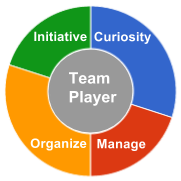
\includegraphics[scale=0.62]{img/personal.png}
%    ~
  \section{Hobbies}
      \href{http://olhares.com/diraol}{\langif{br}{Fotografia}{Photography}}
      Tae-Kwon-Do
\end{aside}%
%
% EXPERIÊNCIA (parte 2)
%
\sectionlang{br}{Experiência - cont.}
\sectionlang{en}{Experience - cont.}
\begin{entrylist}
  \entry
    {\langif{br}{Jul/12 - Fev/15}{Jul/12 - Feb/15}}
    {\langif{br}{Analista de Mídias Digitais}{Digital Media Annalist}}
    {O Estado de S.Paulo S/A}
    {\langif{br}{
         Desenvolvedor na equipe de jornalismo de dados.
       }{
         Main developer of the data driven journalism team.
       } ("\href{http://estadaodados.com}{Estadão Dados}")\\
     \langif{br}{
         Palavras Chave: extração, tratamento, união, processamento, análise e \nohyphens{visualização} de dados.
       }{
         Keywords: Data extraction, scraping, gathering, processing, analysis and \nohyphens{visualization}.
       }\hfill
     \href{http://estadaodados.com}{http://estadaodados.com}
    }
   \entry
    {\langif{br}{Jul/08 - Dez/13}{Jul/08 - Dec/13}}
    {\langif{br}{Administrador de Sistemas voluntário}{Volunteer SysAdmin}}
    {Escritório Piloto - Poli-USP}
    {\langif{br}{
         Implementação e manutenção de rede local (LAN) e website.\\
         Palavras Chave:
       }{
         Design and Setup of local network (LAN) and website.\\
         Keywords:
       }
     OpenLDAP, NFS, apache, XEN, DNS , Drupal.
    }
   \entry
    {\langif{br}{Ago/10 - Ago/11}{Aug/10 - Aug/11}}
    {\langif{br}{Professor de Matemática}{Math Teacher}}
    {ACEPUSP}
    {\langif{br}{
         Curso preparatório para vestibular para \nohyphens{estudantes} de baixa renda.\\
         Palavras Chave: Matemática, Geometria, Trigonometria.
       }{
         University Preparatory course for low income students.\\
         Keywords: Mathematics, Geometry, Trigonometry.
       }
     }
   \entry
    {\langif{br}{Ago/10 - Dez/10}{Aug/10 - Dec/10}}
    {\langif{br}{Voluntário}{Volunteer}}
    {Universidade de São Paulo}
    {\langif{br}{Modelagem de base de dados}%para uma nova versão do Sistema de \nohyphens{Avaliação} de Ensino}%
    {Database modeling}\\% for the new version of the Teaching Evaluation System}\\%
    \href{https://github.com/SuperNovaPOLIUSP}{https://github.com/SuperNovaPOLIUSP}}
   \entry
    {\langif{br}{Jan/09 - Ago/10}{Jan/09 - Aug/10}}
    {\langif{br}{Voluntário}{Volunteer}}
    {Escola de Governo}
    {\langif{br}{Desenvolvimento de website institucional (Joomla)}{Design, development and management of institucional website on Joomla}\\
     \langif{br}{Orientação e mentoria de estudantes do curso de Formação de Governantes}{Orientation and Mentoring of Governor Formation Course Students}}
   \entry
    {\langif{br}{Mar/05 - Jun/06}{Mar/05 - Jun/06}}
    {\langif{br}{Bolsista}{Fellow}}
    {Universidade de São Paulo}
    {\langif{br}{
        Desenvolvedor do primeiro Sistema de Avaliação de Ensino da Escola \nohyphens{Politécnica}.
      }{
        Developer of the first Digital Teaching Evaluation System from Escola \nohyphens{Politécnica} da USP.}}
\end{entrylist}%
%
% PROJETOS
%
\sectionlang{br}{Projetos e Comunidades}
\sectionlang{en}{Projects and Communities}
%\section{Projects}
\textbf{\langif{br}{Radar Parlamentar}{The Parliamentary Radar}} \hfill \href{http://radarparlamentar.polignu.org/}{http://radarparlamentar.polignu.org/}\\
\langif{br}%
{Aplicativo que determina ``semelhanças'' entre partidos \nohyphens{políticos} baseado na análise matemática dos dados de votações de projetos de lei na casa \nohyphens{legislativa}. Existem ainda algumas análises relativas a questões de gênero no Parlamento.\\
Este projeto recebeu 4 premiações desde 2012.}%
{A web application that calculate ``similarities'' between political parties based on legislative houses voting data analysis. There are also some gender analysis from the Parliament. 
This project has been awarded 4 times since 2012.}\\
\langif{br}{Palavras Chave:}{Keywords}: Django/Python, R, Postgres, nginx, ElasticSearch, d3js

\textbf{Transparência Hacker \lang{en}{(\textit{Hacker Transparency})}}\\
\langif{br}%
{Membro da comunidade brasileira Transparência Hacker, que atua nas áreas de Governo Aberto, Transparência Pública, Dados Abertos e afins. A comunidade já criou o Ônibus Hacker, participou da criação do \href{http://blog.openingparliament.org/post/72099651071/a-permanent-hacker-space-in-the-brazilian-congress}{\textbf{Laboratório Hacker do Congresso Nacional}}, influenciou na formulação da Lei de Acesso à Informação e do Marco Civil da Internet, dentre outros.}%
{Member of Brazilian Hacker Transparency community, that advocates for OpenGov, Public Transparency, OpenData, etc. The community created the HackerBus, drove the creation of a \href{http://blog.openingparliament.org/post/72099651071/a-permanent-hacker-space-in-the-brazilian-congress}{\textbf{Congress official HackerLab}}, influenced the Brazilian Public Information Access act and the ``Marco Civil da Internet'', among other projects.}
%
% PUBLICAÇÕES
%
\sectionlang{br}{Publicações}
\sectionlang{en}{Publications}
{\href{http://polignu.org/artigo/twitter-api-elasticsearch-e-kibana-analisando-rede-social}{\textbf{Twitter API, ElasticSearch e Kibana - Analisando a rede social}}\\
\emph{\langif{br}{Tutorial sobre como coletar, processar e analisar dados do Twitter}{Tutorial on how to gather, process and analyze twitter traffic.}}\\}\\
%{\href{http://diraol.polignu.org}{\textbf{DiRaOLinux}}\\
%\emph{\langif{br}{Blog para documentar e compartilhar experiências diárias com software livre}{Blog to document and share daily discovers and issues fixes}}\\}\\
\href{http://polignu.org/administrativo/caderno-polignu-volume-1-software-e-culturas-livres}{\textbf{Caderno do PoliGNU - Vol 1 - Software e Cultura Livres}}\\
\emph{\langif{br}{Material introdutório sobre Software Livre e Cultura Livre}{Introductory material about Free Software and Free Culture (pt-br)}}
%
% NOVA PÁGINA
%
\newpage
\pagenumbering{gobble}% Remove page numbers (and reset to 1)
%
% LATERAL
%
\begin{aside}
~
~
~
  \section{\langif{br}{Outras Tecnologias}{Other Techs}}
    CartoDB
    Django
    Drupal
    Gimp
    Git
    Inkscape
    Mediawiki
    MySQL/MariaDB
    NFS
    Nginx
    OpenLDAP
    OpenFlow
    Postgres
    QuantumGis
    SDN
    Varnish
    Wordpress
    Xen
\end{aside}
%
% CURSOS E CERTIFICAÇÕES
%
\sectionlang{br}{Cursos e Certificações}
\sectionlang{en}{Courses and Certifications}
\begin{entrylist}
  \entry
    {02/2017}
    {Data Science Specialization}
    {\langif{br}{Universidade Johns Hopkins no Coursera}{Johns Hopkins University on Coursera}}
    {\emph{\langif{br}{Estatística Inferencial}{Statistical Inference}}\\
    {\langif{br}{Certificado Verificado: }{Verified Certificate: }\scriptsize{\href{https://coursera.org/verify/C2HZUG2HXQJK}{https://coursera.org/verify/C2HZUG2HXQJK}}}}
  \entry
    {01/2016}
    {Data Science Specialization}
    {\langif{br}{Universidade Johns Hopkins no Coursera}{Johns Hopkins University on Coursera}}
    {\emph{\langif{br}{Modelos de Regressão}{Regression Models}}\\
    {\langif{br}{Certificado Verificado: }{Verified Certificate: }\scriptsize{\href{https://coursera.org/verify/T9LTC73MX62A}{https://coursera.org/verify/T9LTC73MX62A}}}}
  \entry
    {11/2015}
    {Data Science Specialization}
    {\langif{br}{Universidade Johns Hopkins no Coursera}{Johns Hopkins University on Coursera}}
    {\emph{\langif{br}{Pesquisa reprodutível}{Reproducible Research}}\\
    {\langif{br}{Certificado Verificado: }{Verified Certificate: }\scriptsize{\href{https://coursera.org/verify/U5X4J6YSDC}{https://coursera.org/verify/U5X4J6YSDC}}}}
  \entry
    {10/2015}
    {Data Science Specialization}
    {\langif{br}{Universidade Johns Hopkins no Coursera}{Johns Hopkins University on Coursera}}
    {\emph{\langif{br}{Análise Exploratória de Dados}{Exploratory Data Analysis}}\\
    {\langif{br}{Certificado Verificado: }{Verified Certificate: }\scriptsize{\href{https://coursera.org/verify/BCSV3DF2F4}{https://coursera.org/verify/BCSV3DF2F4}}}}
  \entry
    {07/2015}
    {Data Science Specialization}
    {\langif{br}{Universidade Johns Hopkins no Coursera}{Johns Hopkins University on Coursera}}
    {\emph{\langif{br}{Obtenção e Limpeza de Dados}{Getting and Cleaning Data}}\\
    {\langif{br}{Certificado Verificado: }{Verified Certificate: }\scriptsize{\href{https://coursera.org/verify/YFY5YWF3MM}{https://coursera.org/verify/YFY5YWF3MM}}}}
  \entry
    {06/2015}
    {Data Science Specialization}
    {\langif{br}{Universidade Johns Hopkins no Coursera}{Johns Hopkins University on Coursera}}
    {\emph{\langif{br}{Linguagem R}{R Programming}}\\
    {\langif{br}{Certificado Verificado: }{Verified Certificate: }\scriptsize{\href{https://coursera.org/verify/M2NP642ZUE}{https://coursera.org/verify/M2NP642ZUE}}}}
  \entry
    {06/2015}
    {Data Science Specialization}
    {\langif{br}{Universidade Johns Hopkins no Coursera}{Johns Hopkins University on Coursera}}
    {\emph{\langif{br}{As Ferramentas do Cientista de Dados}{Data Scientist’s Toolbox}}\\
    {\langif{br}{Certificado Verificado: }{Verified Certificate: }\scriptsize{\href{https://coursera.org/verify/ELJEYB2D8A}{https://coursera.org/verify/ELJEYB2D8A}}}}
  \entry
    {12/2014}
    {\langif{br}{Objetos Pythonicos}{Pythonic Objects}}
    {\langif{br}{PythonPro}{PythonPro}}
    {\href{https://adm.python.pro.br/cursos}{https://adm.python.pro.br/cursos}}
\end{entrylist}
%
% NOVA PÁGINA
%
\newpage
\pagenumbering{gobble}% Remove page numbers (and reset to 1)
%
% EVENTOS
%
\sectionlang{br}{Eventos}
\sectionlang{en}{Events}
{\footnotesize{\langif{br}{Dez/16}{Dec/16}}} - \href{https://www.facebook.com/events/1617891821849460/}{\textbf{UP\{Design For All\}it}}\\
\langif{br}{Mentor do 3$^o$ encontro \textit{UPWIT - Design For All}. Um evento com objetivo de pensar tecnologias de forma inclusiva}
           {Mentor on the 3$^{rd}$ \textit{UPWIT - Design For All}. An event to think inclusive technologies}.

{\footnotesize{\langif{br}{Mai/16}{May/16}}} - \href{https://rgaiacs.github.io/2016-05-27-ccsl/}{\textbf{Software Carpentry Workshop}}\\
\langif{br}{Instrutor de R no workshop realizado na Universidade de São Paulo (USP)}
           {R instructor on the workshop held at University of São Paulo}.
% http://web.archive.org/web/20170301105603/https://rgaiacs.github.io/2016-05-27-ccsl/

{\footnotesize{\langif{br}{Dez/15}{Dec/15}}} - \href{http://www.lets.go.gov.br/}{\textbf{Hackatona Let's GO}}\\
\langif{br}{Mentor na Hackathona promovida pela Secretaria de Estado de Gestão e Planejamento do Governo de Goiás}
           {Mentor on the Hackathon promoted by Goiás State Government Planning and Management Secretary}.
% http://web.archive.org/web/20160504011426/http://www.lets.go.gov.br/

{\footnotesize{\langif{br}{Out/15}{Oct/15}}} - \href{http://www.hackagenda.com.br/evento/sesi-cultura-digital-2015-hackathon-o-museu-do-seculo-xxi/}{\textbf{SESI Cultura Digital 2015 + Hackathon “O museu do século XXI”}}\\
\langif{br}{Instrutor do workshop ``mapeamento com \textbf{CartoDB}'' e mentor dos grupos participantes do Hackathon}
           {``Mapping with CartoDB'' workshop instructor and Hackathon mentor}.
% http://web.archive.org/web/20170301110629/http://pinghacker.com.br/hackagenda/sesi-cultura-digital-2015-hackathon-o-museu-do-seculo-xxi/
% http://web.archive.org/web/20170301110501/http://www.firjan.com.br/sesi/qualidade-de-vida/projetos-sesi-cultural/sesi-cultura-digital/hackaton/

{\footnotesize{\langif{br}{Set/15}{Sep/15}}} - \href{http://rgaiacs.github.io/2015-09-10-usp/}{\textbf{Software Carpentry Workshop}}\\
\langif{br}{Instrutor de git no workshop realizado na Universidade de São Paulo (USP)}
           {Git instructor on the workshop held at University of São Paulo}.
% http://web.archive.org/web/20160602202812/https://rgaiacs.github.io/2015-09-10-usp/

{\footnotesize{\langif{br}{Ago/15}{Aug/15}}} - \href{https://portaldoaluno.casperlibero.edu.br/agenda-eventos/semana-de-jornalismo-casper-libero-2/}{\textbf{\langif{br}{Seminário de Jornalismo da Faculdade Casper Líbero}{Journalism Seminar on Casper Líbero University}}}\\
\langif{br}{Debatedor na mesa Jornalismo de Dados e Políticas Públicas de Comunicação}
           {Debater a panel about Data Journalism and Public Policies for Communications}.
% https://web.archive.org/web/20170301110810/https://portaldoaluno.casperlibero.edu.br/agenda-eventos/semana-de-jornalismo-casper-libero-2/

{\footnotesize{Jun/15}} - \href{https://setemasters.imasters.com.br/edicoes/design-de-apis/}{\langif{br}{\textbf{7Masters Design de APIs}}{\textbf{7Masters APIs Design}}}\\
\langif{br}{Apresentação: APIs para visualização de dados públicos}%
           {Talk: APIs for open government data visualizations}.
% https://setemasters.imasters.com.br/edicoes/design-de-apis/
% https://web.archive.org/web/20160624032825/http://setemasters.imasters.com.br/edicoes/design-de-apis/
% https://setemasters.imasters.com.br/conversas/apis-para-visualizacao-de-dados-publicos/
% https://web.archive.org/web/20170301120904/https://setemasters.imasters.com.br/conversas/apis-para-visualizacao-de-dados-publicos/

{\footnotesize{Jan/14}} - \href{http://www.techtudo.com.br/noticias/noticia/2014/01/cp2014-campus-party-brasil-2014-guia-traz-principais-atividades-por-perfil.html}{\textbf{\langif{br}{Campus Party Brasil 2014}{2014 Brazil Campus Party}}}\\
\langif{br}{Oficina: ``Dinheiro Público, para onde vai, para onde você quer que vá?''}
           {Workshop: ``Public Budget, where does it go, where do you want it to go to?''}
% https://web.archive.org/web/20150517063722/http://www.techtudo.com.br/noticias/noticia/2014/01/cp2014-campus-party-brasil-2014-guia-traz-principais-atividades-por-perfil.html

{\footnotesize{Nov/13}} - \href{https://knightcenter.utexas.edu/pt-br/blog/00-14390-inscricoes-abertas-para-primeiro-curso-da-anj-com-o-centro-knight-introducao-ao-jornal}{\textbf{\langif{br}{Curso de Introdução ao Jornalismo de Dados}{Introduction to Data Journalism MOOC}}}\\
\langif{br}{Instrutor do módulo ``Programação''. Curso organizado pelo Knight Center e pela \nohyphens{Associação} Brasileira de Jornais}
           {``How to code'' module instructor. Course organized by Knight Center and the Brazilian National Journals Association}.
%https://web.archive.org/web/20170301112535/https://knightcenter.utexas.edu/pt-br/blog/00-14390-inscricoes-abertas-para-primeiro-curso-da-anj-com-o-centro-knight-introducao-ao-jornal

{\footnotesize{Nov/13}} - \href{https://web.archive.org/web/20140330181037/http://2.encontro.dados.gov.br/encontro.html}{\textbf{\langif{br}{II Encontro Nacional de Dados Abertos}{II Brazilian National Conference of OpenData}}}\\
\langif{br}{\textit{Chairman} da Trilha de Visualização de Dados}
           {Dataviz trail Chairman}.
% http://2.encontro.dados.gov.br/encontro.html

{\footnotesize{Jul/13}} - \href{http://abraji.org.br/congresso/}{\textbf{\langif{br}{9$^o$ Congresso Internacional de Jornalismo Investigativo}{9$^{th}$ International Investigative Journalism Congress}}}\\
\langif{br}{Instrutor do workshop ``Programação para Jornalistas''}
           {``Coding for journalists'' workshop instructor}.

{\footnotesize{Jul/13}} - \href{http://rodadahacker.com/}{\textbf{II RodAda Hacker}}\\
\langif{br}{Mentor na segunda edição da ``RodAda Hacker, um workshop de um dia que objetiva promover autonomia  tecnológica a mulheres}%
           {Mentor on the second edition of ``RodAda Hacker'', a one day workshop that aims to promote women technological autonomy}.

{\footnotesize{\langif{br}{Mai/13}{May/13}}} - \href{http://www2013.org/}{\textbf{www2013 Conference}}\\
\langif{br}{Palestrante na mesa ``\textit{eGov and Open Data Camp}'', falando sobre ``\textit{The challenges and opportunities of data journalism}''}
           {Speaker on the ``eGov and Open Data Camp'' panel, talking about ``The challenges and opportunities of data journalism''}.
% https://web.archive.org/web/20161223084334/http://www2013.org/tracks/w3c-track/

{\footnotesize{\langif{br}{Abr/13}{Apr/13}}} - \href{https://setemasters.imasters.com.br/edicoes/opendata/}{\textbf{7Masters OpenData}}\\
\langif{br}{Apresentação do projeto Radar Parlamentar.}
           {Speech about the Parliamentary Radar Project}.
% https://setemasters.imasters.com.br/edicoes/opendata/
% https://web.archive.org/web/20140923074920/http://setemasters.imasters.com.br/edicoes/opendata/
% https://setemasters.imasters.com.br/conversas/radar-parlamentar/
% https://web.archive.org/web/20170301120109/https://setemasters.imasters.com.br/conversas/radar-parlamentar/

{\footnotesize{Mar/13}} - \href{http://rodadahacker.com/}{\textbf{I RodAda Hacker}}\\
\langif{br}{Mentor na primeira edição da ``RodAda Hacker, um workshop de um dia que objetiva dar a mulheres mais autonomia com tecnologias}%
           {Mentor on the first edition of ``RodAda Hacker'', a one day workshop that aims to give woman autonomy with technologies}.

{\footnotesize{Nov/12}} - \href{http://hackshackers.com/blog/author/gfaleiros/}{\textbf{\langif{br}{1$^o$ Hackathon HacksHackers}{1$^{st}$ HacksHackers Hackathon}}}
% https://web.archive.org/web/20160414124730/http://hackshackers.com/blog/author/gfaleiros/

{\footnotesize{\langif{br}{Out/12}{Oct/12}}} - \href{http://yapcbrasil.org.br/2012/talk/110}{\textbf{YAPC::Brasil 2012}}\\
\langif{br}{Palestrante: ``Radar Parlamentar: Desvendando a política legislativa''}%
           {Speaker: ``The Parliamentary Radar: Unraveling the legislative politics''}.
% https://web.archive.org/web/20121022134231/http://yapcbrasil.org.br/2012/talks

{\footnotesize{Jul/12}} - \href{http://softwarelivre.org/fisl13}{\textbf{\langif{br}{13$^o$ Fórum Internacional de Software Livre (FISL)}{13$^{th}$ International Free Software Forum}}}\\
\langif{br}{Apresentação do Projeto Radar Parlamentar no Workshop de Software Livre (WSL)}
           {Presented the Parliamentary Radar project on the Free Software Workshop (WSL)}.
% http://softwarelivre.org/articles/0125/7499/caderno-digital.pdf

{\footnotesize{\langif{br}{Mai/10}{May/10}}} - \href{http://artigo19.org/infoedireitoseu/?p=560}{\textbf{\langif{br}{O direito ao Acesso à Informação}{The Right to Information Access}}}\\
\langif{br}{Palestrante sobre o Direito ao Acesso à Informação num debate na PUC-SP}%
           {Speaker on the ``Right to Information Access'' debate at PUC University}.
% https://web.archive.org/web/20170120024235/http://artigo19.org/infoedireitoseu/?p=560

%
%\\
%
%\begin{flushleft}
%\emph{November 22th, 2014}
%\end{flushleft}
%\begin{flushright}
%
%\end{flushright}
%
%%% This piece of code has been commented by Karol Kozioł due to biblatex errors. 
% 
%\printbibsection{article}{article in peer-reviewed journal}
%\begin{refsection}
%  \nocite{*}
%  \printbibliography[sorting=chronological, type=inproceedings, title={international peer-reviewed conferences/proceedings}, notkeyword={france}, heading=subbibliography]
%\end{refsection}
%\begin{refsection}
%  \nocite{*}
%  \printbibliography[sorting=chronological, type=inproceedings, title={local peer-reviewed conferences/proceedings}, keyword={france}, heading=subbibliography]
%\end{refsection}
%\printbibsection{misc}{other publications}
%\printbibsection{report}{research reports}

\end{document}
